\chapter{Тематика и социальные сети радиостанций}
\label{ch:radio-station}

Радиостанции --- комплекс устройств и сооружений, служащих для подготовки программ радиовещания. 
Эта глава посвящена исследованию программ радиовещания, 
анализируется объект Викиданных \wdqName {<<вещательная радиостанция>>}{14350} и его свойства. 
Получен список всех радиостанций, описанных в Викиданных. 
С помощью запросов получено количество радиостанций у различных стран, 
определены подклассы радиостанций. 
Найдены радиостанции, вещательные каналы и~СМИ в~СССР и~России, 
выделены группы тематической направленности, 
представлены аккаунты в~социальных сетях.

\section{Число радиостанций по странам}

Получим список всех радиостанций с~указанием страны, к которой они относятся, 
посредством свойства \wdProperty{495}{<<страна происхождения>>}. 
Запрос~\ref{lst:all_radio_stations} вернул около 100 станций, 
что является недостаточным числом для радиовещательных программ всего мира, представленных в Викиданных.

\begin{lstlisting}[ 
    language=SPARQL,
    caption={\href{https://w.wiki/5unA}{Cписок всех радиостанций со свойством <<страна происхождения>>}\protect\footnotemark},
    label=lst:all_radio_stations,
    texcl,
    numbers=none
    ]
# List of radio stations and country
SELECT ?radio ?radioLabel ?countryLabel WHERE
{
  ?radio wdt:P31 wd:Q14350; # instance of radio station
         wdt:P495 ?country. # country of origin
  SERVICE wikibase:label { bd:serviceParam wikibase:language "ru,en" }
}
\end{lstlisting}%
\footnotetext{Получено: 118 результатов на 2024 год. 
              Ссылка на SPARQL-запрос: \href{https://w.wiki/9qag}{https://w.wiki/9qag}.}


Посмотрим количество радиостанций у~разных стран в~запросе~\ref{lst:NStationsCountryP495}.
Суммируем число станций в~переменную \lstinline|?sumRadio| 
с~помощью команды \lstinline|COUNT()| в~строке~2. 
Сгруппируем станции по~странам с~помощью команды \lstinline|GROUP BY| в~строке~7.


        \lstset{escapeinside={(*@}{@*)}}
        \sethlcolor{pink}

\begin{lstlisting}[ 
    language=SPARQL,
    caption={\href{https://w.wiki/9qau}
                  {Количество радиостанций со свойством <<страна происхождения>>
                   по странам}\protect\footnotemark},
    label=lst:NStationsCountryP495,
    xleftmargin=18pt,
    numbers=left,
    ]
# Number of radio stations for each country 
SELECT ((*@\hl{COUNT}@*)(?radio) as (*@\hl{?sumRadio}@*)) ?countryLabel WHERE {
  ?radio wdt:P31 wd:Q14350; # is radio station
         wdt:P495 ?country. # has country of origin
  SERVICE wikibase:label { bd:serviceParam wikibase:language "ru,en" }
}
(*@\hl{GROUP BY}@*) ?countryLabel
ORDER BY DESC (?sumRadio)
\end{lstlisting}%
\footnotetext{Получено: 31 страна с радиостанциями на 2024 год. 
              Ссылка на SPARQL-запрос: \href{https://w.wiki/9qau}{https://w.wiki/9qau}.}

Всего в мире около двухсот стран (смотри главу <<\nameref{ch:country}>> 
на~с.~\pageref{ch:RussiaNotCountryPPS}), 
но запрос~\ref{lst:NStationsCountryP495} нашёл только 31 страну с~радиостанциями. 
По-видимому, свойство \wdProperty{495}{<<страна происхождения>>} больше подходит для~указания 
<<страны происхождения творческого произведения или другого продукта>>, 
что и~указано в~описании этого свойства. 


\begin{margintable}
\caption{Страны с наибольшим числом радиостанций на 2024 год}
\begin{tabular}{|c|c|c|}
\hline
\textnumero & Количество & Страна \\
\hline
1 & 15847 & США \\
2 & 1567 & Мексика \\
3 & 1310 & Канада \\
4 & 980 & Филиппины \\
5 & 824 & Великобритания \\
6 & 734 & Бразилия \\
7 & 584 & Германия \\
8 & 464 & Австралия \\
9 & 427 & Франция \\
10 & 371 & Индия \\
\ldots & \ldots & \ldots \\
23 & 87 & Россия \\
\ldots & \ldots & \ldots \\
32 & 55 & Нидерланды \\
\ldots & \ldots & \ldots \\
\hline
\end{tabular}
\label{tab:number_of_radio_stations}
\end{margintable}


Заменив свойство радиостанций <<страна происхождения>> 
на~свойство <<\wdProperty{17}{государство}>> 
в~строке~4 запроса~\ref{lst:NStationsCountryP17}, 
получим уже больше двухсот стран. 

\begin{lstlisting}[ 
    language=SPARQL,
    caption={\href{https://w.wiki/9qdC}
                  {Количество радиостанций со свойством <<государство>>
                   по~странам}\protect\footnotemark},
    label=lst:NStationsCountryP17,
    xleftmargin=18pt,
    numbers=left,
    ]
# Number of radio stations for each country 
SELECT (COUNT(?radio) as ?sumRadio) ?countryLabel WHERE {
  ?radio wdt:P31 wd:Q14350; # is radio station
         (*@\hl{wdt:P17}@*) ?country.  # from country
  SERVICE wikibase:label { bd:serviceParam wikibase:language "ru,en" }
}
GROUP BY ?countryLabel
ORDER BY DESC (?sumRadio)
\end{lstlisting}%
\footnotetext{Получено: 209 стран с~радиостанциями~на 2024 год. 
              Ссылка на SPARQL-запрос: \href{https://w.wiki/9qdC}{https://w.wiki/9qdC}.}

Из~этих двухсот стран в~табл.~\ref{tab:number_of_radio_stations} 
представлены страны с наибольшим числом станций. 
В Нидерландах по~запросу~\ref{lst:NStationsCountryP495} есть 69 станций 
(в~остальных 30 странах меньше десяти станций), 
а~по~запросу~\ref{lst:NStationsCountryP17}~---  всего 55 радиостанций.



\section{Подклассы радиостанций}

Найдём список подклассов радиостанций и размер подкласса 
с~помощью запроса~\ref{lst:subclasses_of_radio_stations}.

\begin{lstlisting}[ 
    language=SPARQL,
    caption={\href{https://w.wiki/9qej}
                  {Список подклассов радиостанций и размер подклассов}\protect\footnotemark},
    label=lst:subclasses_of_radio_stations,
    xleftmargin=18pt,
    numbers=left,
    ]
# List of radio subclasses and subclass sizes
SELECT ?subRadio ?subRadioLabel (COUNT(?r) AS ?count) WHERE 
{
  ?subRadio wdt:P279* wd:Q14350. # subclass of radio station
  ?r wdt:P31 ?subRadio.          # instance of this subclass
  SERVICE wikibase:label { bd:serviceParam wikibase:language "ru,en" }
}
GROUP BY ?subRadio ?subRadioLabel
ORDER BY DESC(?count)
\end{lstlisting}%

\footnotetext{Получено: 23 подкласса радиостанций на 2024 год. 
              Ссылка на SPARQL-запрос: \href{https://w.wiki/9qej}{https://w.wiki/9qej}.}

Из запроса~\ref{lst:subclasses_of_radio_stations} мы получили встречаемые подклассы радиостанций, что помогло нам понять какой подкласс наиболее актуален. 

\marginnote[1\baselineskip]{%
        \label{question:radio}
        \MarginQuestion
        Запрос~\ref{lst:subclasses_of_radio_stations} написан с ошибкой, потому что в результате поиска подклассов радиостанций мы получаем сами \wdqName{<<вещательные радиостанции>>}{14350} . Так почему в списке подклассов мы получаем сами радиостанции? И что необходимо исправить в запросе~\ref{lst:subclasses_of_radio_stations}, чтобы сам класс не попадал в свои подклассы? 
        
        См. ответ на~с.~\pageref{answer:radio_station}.
}

\todoVlad{
Егор, Вы мне задали правильный вопрос, почему в списке подклассов радиостанции мы 
опять получаем радиостанцию, причём это самый большой подкласс, содержит около 30 тыс. объектов.\\

\vspace{12pt}
Напишите на полях этот вопрос
(см. как это сделано в главе про музыку у Владимира, 
ищите команду 
{\textbackslash}MarginQuestion 
 в коде его главе, она отрисовывает настольную лампу).\\ 
И дополните этот вопрос просьбой к читателю, 
чтобы он исправил запрос~\ref{lst:subclasses_of_radio_stations} так, 
чтобы сам класс не попадал в свои подклассы.\\ 
Подсказка: нужно использовать квантификатор +, а не звёздочку *.\\

\vspace{12pt}
И второе, Егор, в разделе <<Ответы>> в конце книги (файл answers) 
напишите ответ на этот вопрос и на эту просьбу (напишите правильный запрос).\\ 
Должны быть перекрёстные ссылки: с вопроса на ответ и обратно. 
Посмотрите, как это сделано у Владимира. }
\answerVlad{Ответ: сделано }




\newpage
\section{Отечественные радиостанции, СМИ и вещательные каналы: UNION против VALUES}

Найдём радиостанции, вещательные каналы и СМИ в СССР и России 
с~помощью запроса~\ref{lst:radioRussiaUNION}. 
Радиостанции не повторяются благодаря команде \lstinline|DISTINCT| в~строке~2. 

Запрос получился достаточно громоздкий из-за использования команды \lstinline|UNION|. 
Перепишем скрипт с~использованием команды \lstinline|VALUES|, 
объединяющей значения (объекты Викиданных) в массив. 
Обычно код с командой \lstinline|VALUES| становится компактнее. 
Запрос~\ref{lst:radioRussiaVALUES} получился короче на одну строку, 
но кажется более простым для понимания, поскольку вся соль скрипта заключена 
в строках 7 и 8. 


\begin{lstlisting}[ 
    language=SPARQL,
    caption={\href{https://w.wiki/9qst}{Список радиостанций, вещательных каналов и СМИ в России, и СССР}\protect\footnotemark},
    label=lst:radioRussiaUNION,
    xleftmargin=18pt,
    numbers=left,
    ]
# List of radio stations, broadcasting and mass media in Russia 
SELECT (*@\hl{DISTINCT}@*) ?radio ?radioLabel WHERE
{
  {?radio wdt:P31 wd:Q14350}    UNION # is radio station OR
  {?radio wdt:P31 wd:Q15265344} UNION # is broadcasting OR
  {?radio wdt:P31 wd:Q11033}          # is mass media
    
  {?radio wdt:P17 wd:Q15180} UNION    # in USSR OR
  {?radio wdt:P17 wd:Q159}            # in Russia
  SERVICE wikibase:label { bd:serviceParam wikibase:language "ru,en" }
}
\end{lstlisting}%
\footnotetext{Получено: 121 радиостанция на 2024 год. 
              Ссылка на SPARQL-запрос: \href{https://w.wiki/9qst}{https://w.wiki/9qst}. }


\begin{lstlisting}[ 
    language=SPARQL,
    caption={\href{https://w.wiki/9quA}{Радиостанции, вещательные каналы и СМИ по России, и по СССР}\protect\footnotemark},
    label=lst:radioRussiaVALUES,
    xleftmargin=18pt,
    numbers=left,
    ]
# List of radio stations, broadcasting and mass media in Russia 
SELECT DISTINCT ?radio ?radioLabel ?mediaTypeLabel ?countryLabel WHERE
{           # radio station, broadcasting, mass media
  VALUES ?mediaType {wd:Q14350 wd:Q15265344 wd:Q11033}
  VALUES ?country {wd:Q15180 wd:Q159} 
              # Soviet Union, Russia
  ?radio wdt:P31 ?mediaType; # is one of mass media
         wdt:P17 ?country.   # related to Soviet Union or Russia
  SERVICE wikibase:label { bd:serviceParam wikibase:language "ru,en" }
}
\end{lstlisting}%
\footnotetext{Получено: 129 радиостанций на 2024 год. 
              Ссылка на SPARQL-запрос: \href{https://w.wiki/9quA}{https://w.wiki/9quA}. }


Одним из преимуществ такого подхода с использованием команды \lstinline|VALUES| 
стало то, что мы можем воспользоваться именами массивов \lstinline|?mediaType| и \lstinline|?country|, 
чтобы вывести на печать вид медиа и страну 
(\lstinline|?mediaTypeLabel| и \lstinline|?countryLabel|) 
в~строке~2 запроса~\ref{lst:radioRussiaVALUES}.

\marginnote[1\baselineskip]{%
        \label{question:radio2}
        \MarginQuestion
	 В выводе запроса~\ref{lst:radioRussiaUNION} мы можем видеть 121 радиостанцию, а в запросе~\ref{lst:radioRussiaVALUES} 129 радиостанций.
        Исходя из результатов можно задаться вопросом: почему имеются различия в запросах, если они выполняют идентичную задачу? 
        
        См. ответ на~с.~\pageref{answer:radio_station2}.
}
 



\todoVlad{
Егор, в запросе~\ref{lst:radioRussiaUNION} с~UNION было 120 станций. 
А после замены на VALUES в запросе~\ref{lst:radioRussiaVALUES}
стало 128 станций.\\
Напишите на поля вопрос об этом (с лампочкой).\\

\vspace{12pt}
В ответе в главе <<Ответы>> попробуйте это объяснить. 
Чтобы понять, в чём дело: найдите примеры станций, которые появляются во втором случае, 
посмотрите на их свойства на Викиданных.}
\answerVlad{Ответ: сделано }





\newpage
\section{Темы отечественных радиостанций и конкатенация строк}

Попробуем понять, какие темы представлены на радиостанциях, СМИ и~вещательных каналах в~СССР и~России 
с~помощью запроса~\ref{lst:SubjRadio}. 

Главные темы радиостанций и других объектов задаются свойством \wdProperty{921}{<<основная тема>>}. 
У~одной станции может быть указано несколько тем, 
см. столбец <<Тема (mainSubject)>> в~табл.~\ref{tab:CONCAT}. 
В этой таблице приведены примеры главных тем для <<Радио Звезда>> и <<Марий Эл Радио>>.

Функция \lstinline|GROUP_CONCAT| (строка~3 запроса~\ref{lst:SubjRadio}) 
объединяет (конкатенирует) строки \lstinline|?subjName|, <<склеивая>> их разделителем, 
здесь~--- запятой с пробелом. 


\begin{margintable}
\centering
\caption{Две радиостанции с примером использования функции \lstinline|GROUP\_CONCAT|, 
         результат записан в переменную ?mainSubject}
%\begin{tabular}{|p{14em}|p{10em}|p{10em}|}
\begin{tabular}{|p{64pt}|p{62pt}|p{96pt}|}
\hline
Объект (radio) & Метка (radioName) & Тема (mainSubject) \\
\hline
\wdqName{Radio Zvezda}{4387399} & Радио Звезда & война, политика, экономика, вооружённые силы, новости, patriot \\
\hline
\wdqName{Mari~El Radio}{30909585}
    \href{Q30909585} & Марий Эл Радио & музыка, комедия, интервью \\
\hline
\end{tabular}
\label{tab:CONCAT}
\end{margintable}


\begin{lstlisting}[ 
    language=SPARQL,
    caption={\href{https://w.wiki/9qwk}
                  {Список тематик радиостанций, СМИ и вещательных каналов}\protect\footnotemark},
    label=lst:SubjRadio,
    xleftmargin=18pt,
    numbers=left,
    ]
# List of the main topics of radio stations, media and mass media
SELECT ?radio ?radioName
       ((*@\hl{GROUP\_CONCAT}@*)(DISTINCT ?subjName;separator=", ") AS ?mainSubjects) WHERE 
{           # radio station, broadcasting, mass media
  VALUES ?mediaType {wd:Q14350 wd:Q15265344 wd:Q11033}
  VALUES ?country {wd:Q15180 wd:Q159} 
              # Soviet Union, Russia
  
  ?radio wdt:P31 ?mediaType; # is one of mass media
         wdt:P17 ?country;   # in country  
         wdt:P921 ?subj.     # has main topic
  
  SERVICE wikibase:label { bd:serviceParam wikibase:language "ru,en".
                           ?radio rdfs:label ?radioName.
                           ?subj  rdfs:label ?subjName. }
} GROUP BY ?radio ?radioName
\end{lstlisting}%
\footnotetext{Получено: 73 тематические группы на 2024 год. 
              Ссылка на SPARQL-запрос: \href{https://w.wiki/9qwk}{https://w.wiki/9qwk}.}

\marginnote[1\baselineskip]{%
        \label{question:radio3}
        \MarginQuestion
В запросе~\ref{lst:SubjRadio} вёлся поиск тематик радиостанций, СМИ и вещательных каналов. Далее была построена таблица~\ref{tab:number_of_topics}. Возможно ли создать граф с вершинами двух типов? Первый тип вершин: вершина соответствует ровно одной главной теме, например, <<медицина>> или <<здоровье>>, или <<юмор>>.  Второй тип вершин: вершина — это радиостанция. Ребро между радиостанцией и какой-либо темой отрисовывается, если эта тема указана в свойствах объекта этого радио на сайте Викиданных.
 }



\todoVlad{
Егор, напишите на поля вопрос (с лампочкой) о том, чтобы читатель построил такой запрос, 
чтобы можно было создать граф с вершинами двух типов:\\ 
(1) вершина соответствует ровно одной главной теме, например, <<медицина>> или <<здоровье>>, или <<юмор>>.\\
(2) вершина~--- это радиостанция. 
Ребро между радиостанцией и какой-либо темой отрисовывается, 
если эта тема указана в свойствах объекта этого радио на сайте Викиданных. 

\vspace{12pt}
Ответ в главе <<Ответы>> не требуется.}
\answerVlad{Ответ: сделано }





\begin{margintable}
\caption{Количество тематик у радиостанций, СМИ и вещательных каналов по убыванию на 2023 год}
\begin{tabular}{|c|c|}
\hline
Количество тематик по & Название тематики \\
 \wdProperty{921}{<<основная тема>>} & \\
\hline
44 & музыка \\
5 & поп-музыка \\
5 & рок \\
3 & TopHit \\
3 & хип-хоп \\
3 & молодёжная музыка \\
3 & джаз \\
\hline
30 & новости \\
15 & политика \\
7 & экономика \\
5 & пропаганда \\
5 & авария \\
5 & проект \\
2 & политическая система России \\
\hline
9 & ток-шоу \\
5 & спорт \\
3 & шутка \\
2 & юмор \\
2 & комедия \\
2 & художественная литература \\
3 & спектакль \\
\hline
\end{tabular}
\label{tab:number_of_topics}
\end{margintable}

Таблица~\ref{tab:number_of_topics} даёт нам представление того, 
какие темы более популярны на радиостациях, а~именно:
\wdqName{музыка}{638}, 
\wdqName{новости}{38926} и \wdqName{политика}{7163}.


\todoVlad{
    Егор, получилась отличная таблица. Добавьте к ней следующий запрос (вместе с листингом), 
    чтобы объяснить откуда она появилась:
\url{https://w.wiki/9rLD}.\\
Обновите данные в таблице в соответствии с этим запросом, возможно где-то цифры немного изменились. 

\vspace{12pt}
Закомментируйте строки 5 и 9 в этом листинге, связанные с Россией, и подсчитайте 
то же самое по всем странам мира. 
Добавьте в эту таблицу последний (третий) столбец с числами тематик по всему миру.\\ 
Поменяйте местами первый и второй столбец. То есть порядок столбцов будет такой:
(1) Название, (2) в России, (3) в мире. 

\vspace{12pt}
Сейчас в таблице темы разделены на три логических блока. Это хорошая идея. 
Здесь текстом напишите пояснение - что это за блоки, какие темы являются лидерами в блоке, 
на скольких радиостанциях есть такие темы. 

\vspace{12pt}
Не нужно писать <<Данная таблица>>. Пишите с помощью команды ref - 
также как Вы это делаете при ссылках на запросы или рисунку. Т.е. будет:
<<В табл. N.N ...>>
}
\answerVlad{Ответ: после комментирования строк, результат изменился незначительно (на 9, 3 и меньше).  Может быть я что-то не так сделал, но это маловероятно }











\newpage
\section{Радиостанции, СМИ и вещательные каналы в социальных сетях}

Данный запрос~\ref{lst:socialNetBubbles} находит аккаунты радиостанций, СМИ и вещательных каналов в социальных сетях.

\begin{lstlisting}[ 
    language=SPARQL,
    caption={\href{https://w.wiki/6fKb}{Аккаунты радиостанций, СМИ и вещательных каналов в социальных сетях}\protect\footnotemark},
    label=lst:socialNetBubbles,
    xleftmargin=18pt,
    numbers=left,
    ]
# Counts the number of radios with social media accounts
#defaultView:BubbleChart
SELECT ?netID ?netIDLabel ?netRelation (COUNT(?network) as ?sumNetwork)
WHERE
{                  # Facebook, Instagram, Telegram, Twitter, VK, YouTube, Zen, SoundCloud, Google ID, Odnoklassniki, Rutube, Spotify
  VALUES ?netRelation {wdt:P2013 wdt:P2003 wdt:P3789 wdt:P2002 wdt:P3185 wdt:P2397 wdt:P8816 wdt:P3040 wdt:P2847 wdt:P5163 wdt:P10152 wdt:P5916}
  
  ?radio wdt:P31 wd:Q14350; # instance of radio station
         wdt:P17 wd:Q159;   # radio from Russia
         ?netRelation ?network. # has social network page

  ?netID wikibase:directClaim ?netRelation.
  
  SERVICE wikibase:label {bd:serviceParam wikibase:language "en"}
} GROUP BY ?netID ?netIDLabel ?netRelation 
ORDER BY DESC(?sumNetwork)\end{lstlisting}%

\footnotetext{Получено: \num{12} результатов на 2023 год. Ссылка на SPARQL-запрос: \href{https://w.wiki/6fKb}{https://w.wiki/6fKb}. }

Объясним строку 12 \lstinline|?netID wikibase:directClaim ?netRelation| и необходимость использования предиката wikibase:directClaim в запросе~\ref{lst:socialNetBubbles}.

Для этого нужно начать с объяснения того, что радиостанции соответствует объект и страница на Викиданных. На этой странице есть подраздел Идентификаторы (Identifiers). В этом подразделе перечислены, в том числе, социальные сети, в которых зарегистрирован объект (здесь радиостанция). Два следующих утверждених из запроса выше (на примере ВКонтакте, которому соответствует идентификатор-свойство P3185):

\begin{lstlisting}
# VALUES ?netRelation ... wdt:P3185
# ?radio ... ?netRelation ?network. \# has social network page
\end{lstlisting}

мы получаем ?netRelation для каждой радиостанции, счетчик ?sumNetwork (здесь для ВКонтакте) увеличивается на один.

Проблема в том, что мы не можем получить имя \lstinline|?netRelationLabel|, поскольку конструкция \lstinline|SERVICE wikibase| не работает для свойств, а только для объектов. Нам помогает свойство \lstinline|wikibase:directClaim|, которое возвращает имя \lstinline|?netID| по свойству \lstinline|?netRelation|.


Пузырьковая диаграмма~\ref{fig:radio_station_acc} построенная запросом~\ref{lst:socialNetBubbles}, показывает количество аккаунтов СМИ и радиостанций в социальных сетях. То есть на рисунке показаны социальные сети, размер круга пропорционален количеству зарегистрированных в них аккаунтов СМИ и радиостанций.

Популярными социальными сетями среди радиостанций, СМИ и вещательных каналов в России на 2024 год стали: 
ВКонтакте~--- 28 аккаунтов; 
Instagram~--- 26 аккаунтов; 
Facebook~--- 25 аккаунтов; 
YouTube~--- 24 аккаунта; 
Twitter~--- 21 аккаунт; 
Telegram~--- 20 аккаунтов. 
Таким образом, самой популярной социальной сетью для СМИ в России стал ВКонтакте.

Следующим шагом будет проведено сравнение количества аккаунтов радиостанций, СМИ и вещательных каналов России и всех стран в социальных сетях. Для этого необходимо закомментировать строку 9~\lstline|wdt:P17 wd:Q159| в запросе~\ref{lst:socialNetBubbles}, которая нужна нам для поиска в России.  Аналогично будет построена пузырьковая диаграмма для всех стран, которую построил запрос~\ref{lst:socialNetBubbles} с закомментированной строкой, о которой говорилось ранее. 

Популярными социальными сетями среди радиостанций, СМИ и вещательных каналов во всех странах на 2024 год стали:
Twitter~---4835 аккаунтов;
Facebook~---2044 аккаунтов;
Instagram~---1514 аккаунтов;
Youtube~---397 аккаунтов;
Telegram~---51 аккаунт;
Вконтакте~---44 аккаунта.
Таким образом, самой популярной социальной сетью для СМИ всех стран стал Twitter.

Глядя на результаты двух диаграмм можно сделать вывод о том, что в шестерка популярных социальных сетей осталась почти неизменной, изменились только позиции. Таким образом во второй диаграмме~\ref{fig:radio_station_acc_all_countries}  верхние строчки заняли социальные сети, имеющие большую популярность во всем мире. Социальные сети, которые разработаны в России заняли места ниже в этой шестерке. 



\index{График!Sunburst diagram}
\begin{marginfigure}[1\baselineskip]
{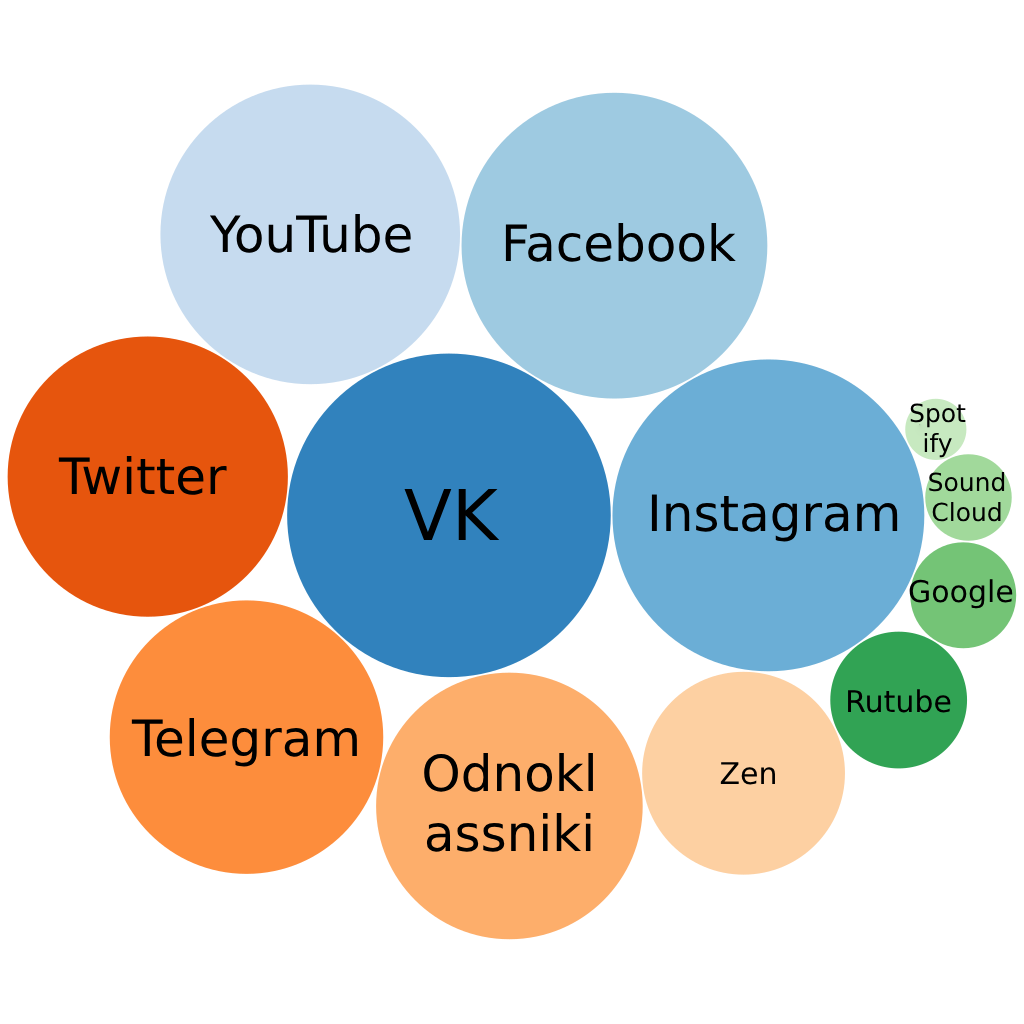
\includegraphics[width=1\linewidth]{chapter/radio_station/Number_of_social_media_accounts_2.png}}
\vspace{-7pt}
\caption{Пузырьковая диаграмма популярности социальных сетей по числу в них аккаунтов радиостанций, СМИ и вещательных каналов на 2024 год}%
\label{fig:radio_station_acc}
\end{marginfigure}

\index{График!Sunburst diagram}
\begin{marginfigure}[1\baselineskip]
{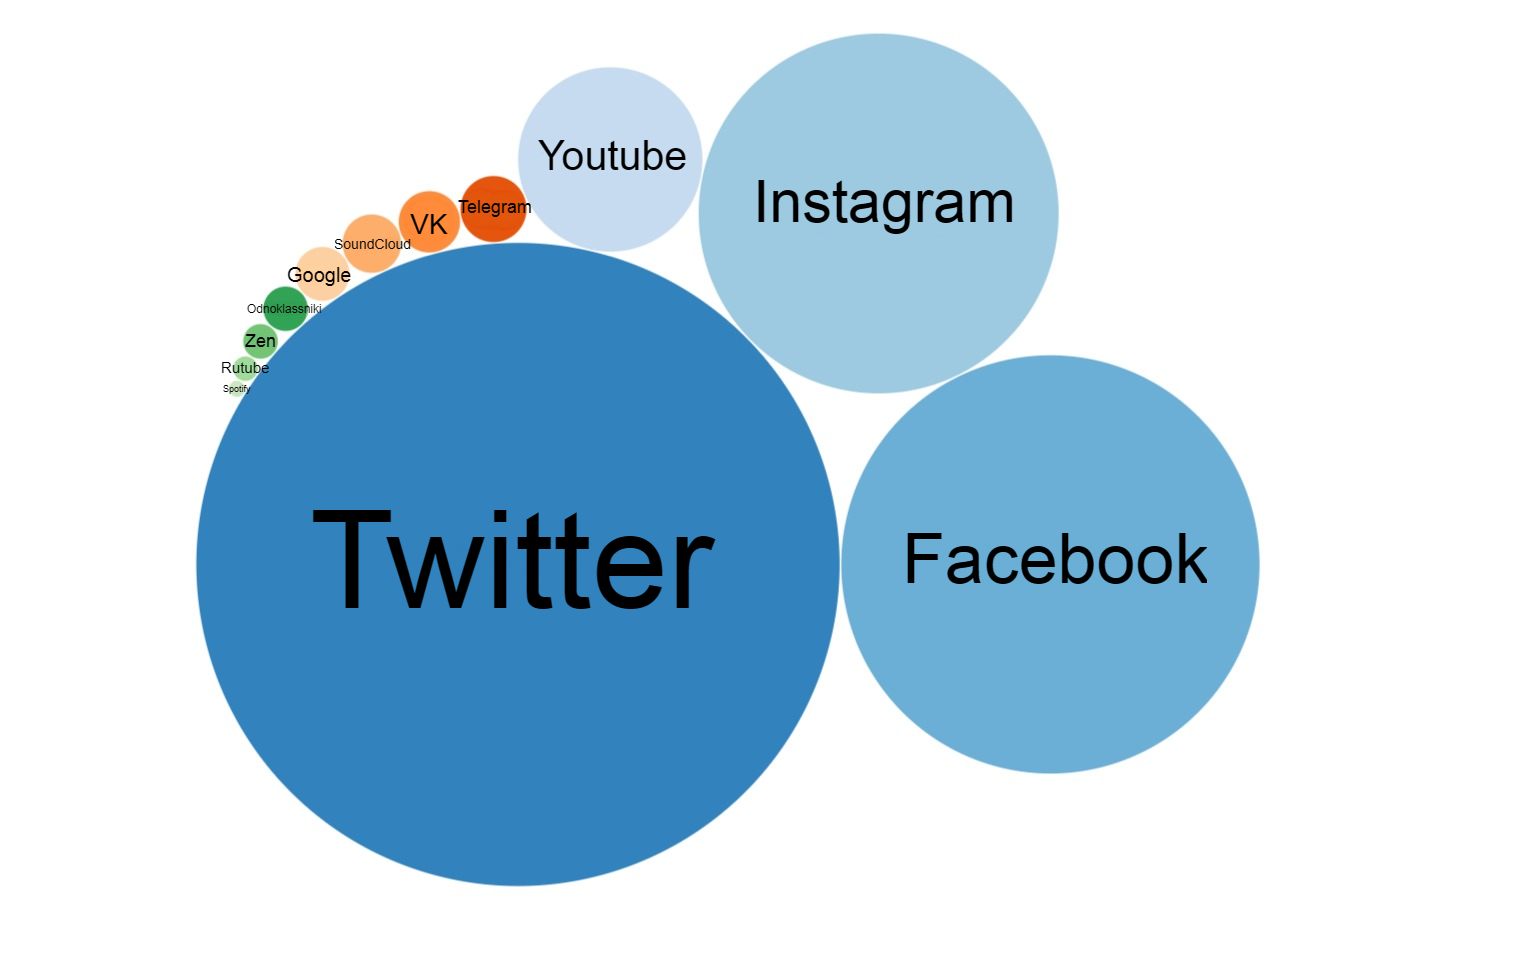
\includegraphics[width=1\linewidth]{chapter/radio_station/Number_of_social_media_accounts_in_all_countries.png}}
\vspace{-7pt}
\caption{Пузырьковая диаграмма популярности социальных сетей по числу в них аккаунтов радиостанций, СМИ и вещательных каналов во всех странах на 2024 год}%
\label{fig:radio_station_acc_all_countries}
\end{marginfigure}


\todoVlad{
Егор, сделайте второй рисунок, 
закомментировав строчку в~запросе~\ref{lst:socialNetBubbles} 
о принадлежности радио к России.\\
Добавьте этот второй рисунок сюда. Напишите словами о разнице между этими двумя диаграммами: про число аккаунтов отечественных радиостанций в соцсетях относительно числа аккаунтов радио всего мира.\\
Второй листинг делать не надо, поскольку он отличается только одной строчкой - 
достаточно в тексте написать - номер строки, которую комментируете.

\vspace{12pt}
Не забудьте при создании картинки отредактировать SVG-файл, чтобы был крупный шрифт для надписей внутри кружков.
}
\answerVlad{Ответ: сделано }
